\pdfinfoomitdate=1
\pdftrailerid{}
\documentclass[11pt]{article}
\usepackage[letterpaper,margin=18mm,top=22mm,bottom=20mm,headheight=15pt]{geometry}
\usepackage{tikz,fancyhdr,amsmath,amssymb,array,booktabs,hyperref,lmodern}
\usepackage[T1]{fontenc}
\hypersetup{hidelinks}\pagestyle{fancy}\fancyhf{}
\fancyhead[L]{\small Week 90 / Sliding number arrays / Adult guide}
\fancyfoot[L]{\small Bellingham Math Circle / Week 90 / W90-FAC-v1}\fancyfoot[R]{\thepage}
\setlength{\parindent}{0pt}\setlength{\parskip}{6pt}
\newcommand{\heading}[1]{\par\textbf{#1}\par}
\begin{document}
\heading{Mathematical overview: a local rule and a global independence theorem}
\textbf{Objects and assumptions.} A Young diagram here has left-justified rows whose lengths do not increase from top to bottom. A skew diagram is an outer such shape with a smaller upper-left diagram removed. Fill its remaining cells with distinct labels $1,\ldots,n$, increasing from left to right and top to bottom. Gray hatched cells form the missing inner diagram; dark crosshatched cells are outside the current outer shape. The open ring marks the one active hole. These are three different states.

\textbf{One slide preserves order and terminates.} A legal starting hole is a southeast corner of the missing inner shape: no missing cell immediately right or below it. Remove that gray piece. Repeatedly move the smaller of the immediate right/below numbered neighbors into the hole, using the sole one when only one exists. When neither exists, remove the final cell from the outer shape. Labels remain distinct and increasing; their count is unchanged. The hole moves only right/down, so a slide ends. One inner missing cell and one outer cell disappear.

\textbf{First fundamental theorem of ordinary jeu de taquin.} Repeating legal whole slides until the inner shape is gone gives the same final \emph{labeled} straight tableau, regardless of which available inner corner starts each slide. This includes the labels, not merely the shape. Within a slide the neighbor choice is deterministic. The theorem does not apply to arbitrary holes, arbitrary masks, repeated labels with an unspecified tie rule, or the shifted/edge-labeled variants in the source.

\textbf{What the finite investigations establish.} Enumerating all legal start choices for one board proves independence for that board. Enumerating every filling and order for one small shape proves it for that finite family. This supplies evidence for, not a proof of, the universal theorem. Its general proof is substantially deeper and is an attributed adult continuation. Elementary proofs remain available for preserved order, termination and complete small-case catalogs.

\textbf{Reversing one recorded slide.} If the original starting cell and deleted exit cell are known, insert the hole at the exit and repeatedly move the larger immediate up/left neighbor into it, stopping at the original cell. This reverses that slide. The final rectification alone does not determine its starting skew array or all its history: different starts can have the same output. Boundary markers carry essential information.

\textbf{Readiness map.} Grades 2--3 may operate supplied one-hole boards after a short demonstration and a check that children retain the comparison rule. Grades 4--5 can design starts, sort full labeled outputs, pool cases, choose whole-slide orders and explain local invariants. No K--1 packet is claimed. An interested younger child may try a one-hole board only if they compare labels and choose moves themselves; otherwise use a familiar different activity. Reading and final recording can be adult-supported; adults should not operate every move. All procedures, timing and materials remain physically untested and unpiloted.
\newpage
\heading{Preparation and a first visit}
Per pair, prepare a reusable $4\times 4$ grid with 30 mm cells, numbered 26 mm tiles 1--5, one 26 mm open-ring hole marker, three gray hatched missing pieces and eight dark crosshatched outside pieces. The shape-specific working inserts show initially outside cells permanently: loose dark pieces cover new exits, not every outside square on a blank board. Keep gray, dark and ring distinguishable in grayscale. Each supplied start has a reset diagram with labels and both masks; do not ask children to reconstruct an old state from memory.

For four middle children and the upper trio, three kits suffice: three grids, fifteen numbered tiles, three rings, nine gray and 24 dark pieces. Prepare two middle pairs and one upper trio; the trio rotates slider, checker and recorder. One adult stays at each table. A separate familiar activity is appropriate for the K--1 table; optional assisted one-hole participation is not a complete younger-table plan. Print only the selected task pages and their matching reset cards and board inserts, one set per kit. Material pages 1--4 are the A, B, D and demonstration boards; page 5 supplies pieces; page 6 has A cards; page 7 D cards; pages 8--10 B cards; page 11 blank grouping cards. Reuse the same kit across visits. Print US Letter, single-sided, Actual Size. The 30 mm grid and 26 mm pieces leave handling clearance; compact task diagrams are references.

Initial preparation is estimated at 20--30 minutes with reusable boards, but physical assembly, mask handling and resets have not been rehearsed. Before classroom use, test a smaller-right choice, a smaller-below choice, a one-neighbor move and terminal removal. Then reset from a card and complete two successive slides, checking that unchosen gray pieces stay and that old exits remain dark. Confirm tiles move easily and the ring does not obscure neighboring labels. A digital trace cannot establish this physical readiness.

\textbf{Launch together.} After five minutes of movement, give two minutes to handle numbers and the ring. Explain the purpose: ``We will slide numbers into a missing corner and compare the shapes that result.'' Use the small non-task board with missing top-left,2 at top-right,1 bottom-left,3 bottom-right. Remove the gray piece and place the ring. Ask which immediate right/below neighbor is smaller. Move 1 up, leaving the ring at bottom-left; move 3 left into it; cover the now-empty bottom-right exit dark. Show the complete output, not just the first swap. The partner checks a move by pointing to the only eligible neighbors. Numbered pieces slide toward the hole; the hole moves right/down.

Work 25--35 minutes with supplied one-hole boards and child-designed increasing starts. Children choose placements and comparisons while adults may read and save one final board. If adults repeatedly rescue every move, remain at one-hole play rather than introduce more masks. Before resetting for a second run, save one final labeled-board sketch on a blank grouping card or the adult whiteboard. Then compare that record with the second finish. The first visit may end by sharing two different starts with the same final shape. Distinguish shape from the full labeled result.

\textbf{A later launch for multiple missing cells.} Show which gray corners have no gray cell immediately right or below. Choose only one, complete its whole slide and remove its exit before selecting a new corner. Keep the unchosen missing squares visible. When comparing orders, reset every label and mask from the same unchanged card. Divide the finite case collection among pairs and pool outcomes; children need not duplicate every run. Reversal gets its own full operation example and both endpoint markers. Allow these as separate visits; finishing the packet is not a goal.
\newpage
\heading{Problems 1--2: one missing corner and a complete small collection}
\textbf{First route.} Student pages 1--2 and material pages 1,5,6 suffice for the A investigation; add material page 4 for the whole-group example. Begin with Problem 1. Problem 2 can fill the remainder of a visit or be a return visit. Children need not perform all five starts before they begin grouping their answers.

\textbf{1. Three starts.} A1 finishes as two rows of length two; A3 and A5 finish as rows of lengths three and one. A3 and A5 have the same outline but different labels. Use a single final-board sketch or place the unchanged start card in a labeled group; a move transcript is unnecessary. A child may slide a tile with a finger first, then move the ring. Only immediate right/below numbered neighbors are candidates.

\textbf{2. Complete A catalog.} The full results are below. A slash separates consecutive rows, all left justified. For example $12/34$ means top row 1,2 and bottom row 3,4.
\begin{center}\begin{tabular}{ccl}\toprule
card&finished rows&outline\\\midrule
A1&$12/34$&$(2,2)$\\
A2&$13/24$&$(2,2)$\\
A3&$134/2$&$(3,1)$\\
A4&$123/4$&$(3,1)$\\
A5&$124/3$&$(3,1)$\\\bottomrule
\end{tabular}\end{center}
These five starts are all possible. Name the top middle and right cells $a,b$, and the bottom left and middle cells $c,d$. Increase requires $a<b$, $a<d$, $c<d$. The smallest label is at $a$ or $c$. If $a=1$, the remaining labels can be put at $b,c,d$ in three orders with $c<d$. If $c=1$, then $a=2$ and the last two labels may be exchanged between $b,d$: two more. Thus $3+2=5$. Children can demonstrate this by placing 1 and sorting the remaining cards, without naming variables.

Hints: which cells could hold 1? If 1 is fixed, which comparison is still free? Make the grouping concrete with the supplied movable cards. Full coverage is a collective task: pairs can own cases and pool them. The finished labeled arrays here are all distinct, even though several have the same outline. This is worth distinguishing before the later preimage question.

\textbf{Readiness.} Grades 2--3 may concentrate on operating and grouping A starts. Completeness and the reason that no other start exists are optional upper-table discussion. Routine adult reading and saving a final result are appropriate; adult choice of every move means the operating rule is not yet independent.
\newpage
\heading{Problem 3: choosing whole slides from one unchanged start}
The D shape has missing cells at top left, top middle and middle left; its labels lie on the descending diagonal. Any order of 1,2,3 along that diagonal is increasing, because no two share a row or column. Hence its six supplied cards are the complete collection.

There are exactly two legal full corner orders: upper, lower, then top left; or lower, upper, then top left. Once the first corner is chosen, the second is forced. Each slide itself has no choice: use the smaller immediate neighbor. Complete a slide and cover its exit before selecting the next missing corner. Reset all labels and masks from the unchanged card before trying the other order.

\begin{center}\begin{tabular}{ccl}\toprule
card&diagonal labels&finished rows, either order\\\midrule
D1&123&$1/2/3$\\
D2&132&$13/2$\\
D3&213&$12/3$\\
D4&231&$12/3$\\
D5&312&$13/2$\\
D6&321&$123$\\\bottomrule
\end{tabular}\end{center}
Each of these six starts gives exactly the same labeled result under the two choices. Checking all twelve complete runs proves this finite statement. It does not prove that every larger skew array is independent of all legal choices. The ordinary rectification theorem says that it is, under the assumptions stated in the overview; the general theorem is attributed background.

Hints: keep unchosen gray pieces visible; compare the same card with itself under two orders; place cards with equal outputs together only after both runs are complete. Ask whether ``the same'' means just the outline or every label in the same cell. If masks and resets require repeated rescue, use one D card as a shared table investigation and revisit the rest later.

\textbf{Demonstration check.} The printed multi-hole example has outer rows $(3,2)$ and missing rows $(2,1)$, with 1 at top right and 2 at bottom middle. Opening the lower missing corner moves 2 left; its old cell becomes the covered exit. The two upper gray cells have stayed unchanged. The next legal corner is the upper middle cell, opened in the fourth image. This demonstrates one complete slide and the next legal start, without silently changing the initial input.

\textbf{Return route.} Problem 3 uses student page 3, material D board page 3, pieces page 5 and D catalog page 7. It can occupy a whole later visit. Problem 6 then reuses the same cards to reverse the question: which starts share one finished arrangement?
\newpage
\heading{Problem 4: design a start for a chosen finish}
This route reverses the direction of the question before requiring the full B catalog. Arrange 1--5 on the blank skew board, increasing in rows and columns, so that ordinary sliding reaches each target outline. A successful example for each target is enough; children need not locate every possible start yet. Use student page 4, B board (material page 2), pieces (page 5), and blank grouping cards (page 11) to save a construction. Keep the B catalog in reserve if children want an independent search first.

Here are three witness starts. Gray squares are missing; each small diagram uses the same B boundary. Card names link the examples to the later complete collection, but a child can build the placements directly.
\begin{center}
\begin{minipage}{0.31\textwidth}\centering B8 / target $(3,2)$
\par\smallskip
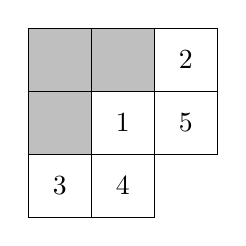
\begin{tikzpicture}[x=8mm,y=-8mm]
\filldraw[fill=black!25,draw=black] (0,0) rectangle ++(1,1);
\filldraw[fill=black!25,draw=black] (1,0) rectangle ++(1,1);
\filldraw[fill=white,draw=black] (2,0) rectangle ++(1,1);
\node at (2.5,0.5) {2};
\filldraw[fill=black!25,draw=black] (0,1) rectangle ++(1,1);
\filldraw[fill=white,draw=black] (1,1) rectangle ++(1,1);
\node at (1.5,1.5) {1};
\filldraw[fill=white,draw=black] (2,1) rectangle ++(1,1);
\node at (2.5,1.5) {5};
\filldraw[fill=white,draw=black] (0,2) rectangle ++(1,1);
\node at (0.5,2.5) {3};
\filldraw[fill=white,draw=black] (1,2) rectangle ++(1,1);
\node at (1.5,2.5) {4};
\end{tikzpicture}\end{minipage}
\begin{minipage}{0.31\textwidth}\centering B3 / target $(3,1,1)$
\par\smallskip
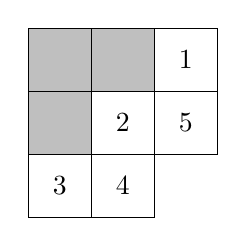
\begin{tikzpicture}[x=8mm,y=-8mm]
\filldraw[fill=black!25,draw=black] (0,0) rectangle ++(1,1);
\filldraw[fill=black!25,draw=black] (1,0) rectangle ++(1,1);
\filldraw[fill=white,draw=black] (2,0) rectangle ++(1,1);
\node at (2.5,0.5) {1};
\filldraw[fill=black!25,draw=black] (0,1) rectangle ++(1,1);
\filldraw[fill=white,draw=black] (1,1) rectangle ++(1,1);
\node at (1.5,1.5) {2};
\filldraw[fill=white,draw=black] (2,1) rectangle ++(1,1);
\node at (2.5,1.5) {5};
\filldraw[fill=white,draw=black] (0,2) rectangle ++(1,1);
\node at (0.5,2.5) {3};
\filldraw[fill=white,draw=black] (1,2) rectangle ++(1,1);
\node at (1.5,2.5) {4};
\end{tikzpicture}\end{minipage}
\begin{minipage}{0.31\textwidth}\centering B1 / target $(2,2,1)$
\par\smallskip
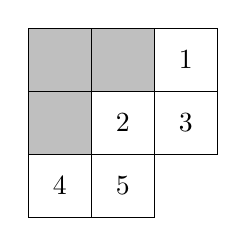
\begin{tikzpicture}[x=8mm,y=-8mm]
\filldraw[fill=black!25,draw=black] (0,0) rectangle ++(1,1);
\filldraw[fill=black!25,draw=black] (1,0) rectangle ++(1,1);
\filldraw[fill=white,draw=black] (2,0) rectangle ++(1,1);
\node at (2.5,0.5) {1};
\filldraw[fill=black!25,draw=black] (0,1) rectangle ++(1,1);
\filldraw[fill=white,draw=black] (1,1) rectangle ++(1,1);
\node at (1.5,1.5) {2};
\filldraw[fill=white,draw=black] (2,1) rectangle ++(1,1);
\node at (2.5,1.5) {3};
\filldraw[fill=white,draw=black] (0,2) rectangle ++(1,1);
\node at (0.5,2.5) {4};
\filldraw[fill=white,draw=black] (1,2) rectangle ++(1,1);
\node at (1.5,2.5) {5};
\end{tikzpicture}\end{minipage}
\end{center}
B8 finishes as $125/34$, B3 as $145/2/3$, and B1 as $13/25/4$, with a slash separating rows. These witness each requested outline. Each has the same labeled output under either available first gray corner; the complete table on the next guide page records both full runs for every start.

Do not impose an arbitrary fixed first corner on the construction task. The ordinary rule already determines each move within a slide. Children can choose a legal first corner and test their proposed placement. Save a successful starting placement, then design another for a different target. This is a search question, not a requirement to perform all 32 catalog trials before making a choice.

Hints, if needed: first check whether the proposed start increases; follow the smallest tile through one full attempt; compare two starts differing by a permissible exchange. A label swap is not automatically legal: recheck the row and column comparisons before sliding. If a child finds more than one start for a target, preserve those cases for the pooled catalog rather than making them redo an identical run.

The next investigation asks whether the collection is complete and classifies all possibilities. Its table shows there are no other final outlines for this specific B input shape. That finite conclusion depends on complete case coverage. The three witnesses alone prove only that the three displayed targets can be reached.
\newpage
\heading{Problem 5: sixteen starts and three final shapes}
The B board is outer shape $(3,3,2)$ with missing shape $(2,1)$. Label its five available cells, in reading order, $a,b,c,d,e$: top right; middle middle and right; bottom left and middle. Its comparisons are $a<c$, $b<c$, $b<e$, $d<e$. The smallest label is at $a,b$ or $d$. These choices give 5,6 and 5 starts, respectively. For $a=1$, choose $b$ next (three completions) or $d$ next (two); for $b=1$, interleave the chains $a<c$ and $d<e$ in six ways; for $d=1$ use the symmetric five-case argument. Thus there are exactly 16.

The two whole-slide orders are the same corner orders as for D. Both give these results:
\begin{center}\begin{tabular}{ccl@{\qquad}ccl}\toprule
card&finished rows&shape&card&finished rows&shape\\\midrule
B1&$13/25/4$&$(2,2,1)$&B9&$124/3/5$&$(3,1,1)$\\
B2&$14/25/3$&$(2,2,1)$&B10&$125/3/4$&$(3,1,1)$\\
B3&$145/2/3$&$(3,1,1)$&B11&$13/24/5$&$(2,2,1)$\\
B4&$134/2/5$&$(3,1,1)$&B12&$135/24$&$(3,2)$\\
B5&$135/2/4$&$(3,1,1)$&B13&$123/4/5$&$(3,1,1)$\\
B6&$12/35/4$&$(2,2,1)$&B14&$123/45$&$(3,2)$\\
B7&$12/34/5$&$(2,2,1)$&B15&$134/25$&$(3,2)$\\
B8&$125/34$&$(3,2)$&B16&$124/35$&$(3,2)$\\
\bottomrule\end{tabular}\end{center}
The $(2,2,1)$ group is B1, B2, B6, B7, B11 (five cards); $(3,1,1)$ is B3, B4, B5, B9, B10, B13 (six); $(3,2)$ is B8, B12, B14, B15, B16 (five). Every final labeled tableau in this table is different. Different outlines and different labeled results answer different questions.

Let pairs share the 16 cards and pool checkable results. Each assigned card needs two full runs from the same reset, not two partially changed states. The table checks all 32 complete runs; its scope is this finite family. It is legitimate to revisit a subset first and finish the catalog another day. Adults can hold the pooled record; children should retain the placement and comparison choices.

Hints: first separate starts by where 1 sits; sort final outlines before investigating labels; use the blank grouping cards instead of repeatedly copying starts. Student page 5 and material pages 2,5,8--11 support this visit. The preparation includes cutting the supplied cards; printing an entire catalog is not a demand that each child transcribe it.
\newpage
\heading{Problems 6--7: preimages and reversing a recorded slide}
\textbf{6. Which start made this target?} The target $13/2$ has D2 and D5; $12/3$ has D3 and D4; the vertical $1/2/3$ has only D1; the horizontal $123$ has only D6. Thus a final arrangement need not reveal its starting card. For this B catalog the answer to the last question is no: all 16 final labeled arrays are different, as the complete table shows. The D counterexamples disprove universal uniqueness; the B finite result does not restore it in general.

Place the unchanged cards beside the actual targets on the tabletop; the printed target area is not a fitted card mat. The operation already has a purpose: discover how much starting information is lost. A child who groups only by outline will merge the two bent three-cell targets incorrectly. Compare all label positions.

\textbf{7. Undo one recorded whole slide.} Coordinates here are (row,column), starting at 1 at the top left. Record S before opening it and E before covering the exit. The forward moves below list the labels moved; reverse moves occur in the opposite order.
\begin{center}\begin{tabular}{cccl}\toprule
start&S&E&forward labels / reverse labels\\\midrule
A2&$(1,1)$&$(1,3)$&1,3 / 3,1\\
A4&$(1,1)$&$(2,2)$&1,4 / 4,1\\
B4 upper&$(1,2)$&$(2,3)$&1,4 / 4,1\\
B4 lower&$(2,1)$&$(3,2)$&2,5 / 5,2\\\bottomrule
\end{tabular}\end{center}
Each backward run restores every label and both boundaries exactly. For B4 reset from the original card before choosing the other starting corner; the problem asks about one slide, not a full rectification before reversal. Uncover the known exit, use the larger immediate up/left neighbor, and stop at the known original corner. Restore its gray missing piece. S and E can sit just outside the cell corners, keeping the numbered space clear.

Why larger? Suppose the last forward move came from the right. Its label now sits left of the hole; any other backward candidate is above the hole. That other tile was not previously on the southeast-moving path, and originally lay above the moved tile, so it is smaller. The case of a last move from below is symmetric: the alternative candidate originally lay left of the moved tile and is smaller. Thus the larger backward candidate undoes the last move. Repeat on the restored earlier state to recover the entire path. This argument assumes an actual legal forward slide and its endpoints. It does not promise reconstruction from an arbitrary final array, arbitrary endpoints, or a rectification with no saved history.

The printed backward demonstration returns the finished $12/3$ array to missing top-left with 2 top-right, 1 bottom-left and 3 bottom-right. It reopens the bottom-right exit, moves 3 right, then 1 down and replaces the original corner with gray. Reversing a recorded slide preserves information; forgetting all boundaries after many slides may not.

Hints: mark both endpoints before removing anything; ask which of the two available up/left labels could have moved last; stop at S even if another neighboring label exists. This is a separate return visit after children can perform and reset a forward slide independently.
\newpage
\heading{Problems 8--9: why the rule matters}
\textbf{8. The larger-neighbor variation.} Every A start loses increasing order. Its resulting rows are:
\begin{center}\begin{tabular}{ccl}\toprule
card&finished rows&one violated comparison\\\midrule
A1&$312/4$&top row $3>1$\\
A2&$213/4$&top row $2>1$\\
A3&$214/3$&top row $2>1$\\
A4&$243/1$&first column $2>1$\\
A5&$24/13$&first column $2>1$\\\bottomrule
\end{tabular}\end{center}
So no A card still finishes increasing under this altered rule. The experiment is a complete finite check, not a claim about every possible board: a board with only one eligible neighbor at every step is unchanged by choosing ``larger.'' One counterexample suffices to show that the altered rule does not preserve increasing arrays universally.

At a hole with right and lower candidates, the larger choice places a larger label above or left of the unchosen smaller one. That introduces an inversion immediately. The A catalog shows the inversion remains in each final result. Compare the two immediate candidates; do not blame a distant tile or allow a diagonal move to repair the altered process.

\textbf{9. What cannot happen under the usual rule?} No label is lost: each swap moves one numbered tile into the unique hole, leaving a unique hole behind; the removed exit is empty. No new label is added and none is duplicated. The count stays fixed through every whole slide and through rectification.

A slide cannot continue forever. Each move takes the hole one row down or one column right. The sum of its row and column therefore increases by exactly one and is bounded on a finite board. When neither candidate exists, the hole is at an outer corner and its empty cell is deleted. Each whole slide also removes one inner missing cell, so finitely many slides finish rectification.

Increasing order is preserved, including comparisons across the one hole. Suppose a tile $x$ moves left. Its new left neighbors were already smaller in its row. If it has a new neighbor $u$ above, the cell immediately right of $u$ contains a tile $v$: the skew boundaries ensure that cell exists when $u$ does. Before the move, row and column order give $u<v<x$. The smaller-candidate rule makes $x$ less than the unchosen lower neighbor when both candidates exist, and farther rightward labels were already larger. For a tile moving up, transpose rows and columns. All comparisons away from the filled hole or across the newly vacated cell follow from the previous order. This induction proves every move preserves increasing labels. Children can point to the three-cell corner instead of using letters. The local argument is separate from the deeper independence-of-corner-orders theorem.

Hints: give one child responsibility for the ring and another for checking its adjacent inequalities; mark the ring's successive positions on spare paper only if a path explanation is needed. Children need not keep a move log while playing. Loss, order and termination are three separate claims, each with its own reason. A few successful examples support a conjecture; the invariant and bounded-motion arguments explain all boards under the stated rules.
\newpage
\heading{Sources, scope and future visits}
Colleen Robichaux, Harshit Yadav and Alexander Yong, \emph{Equivariant cohomology, Schubert calculus, and Edge labeled tableaux}, arXiv:1908.11224v1, Section 3, gives ordinary rules J1/J2 and the first fundamental theorem (Theorem 3.1). Theorem 3.3 and Example 3.4 discuss preimages. Only the ordinary distinct-label setting is used here. Edge-labeled, shifted and repeated-label variants are outside this packet. The source and exact citation are recorded in the editable package; no whole external paper is bundled.

The large theorem says the final labeled tableau is independent of the legal corner choices for every ordinary skew standard tableau. Its general proof is advanced adult background. Our A, D and B enumerations prove the stated finite collections. Children can prove local order preservation, termination, the counts 5,6,16, and nonunique preimages with concrete cases. Do not label a pooled experiment a universal proof.

Week 1 extensions use standard-tableau counting for order-ideal histories (42 and 14 cases). This family asks a different question: sliding skew shapes, selecting whole-slide orders, recovering information and changing a local rule. It does not repeat the earlier counting route. Current Weeks 92--97 do not supersede these questions. The preparation remains substantial but reusable; no forced K--1 worksheet is claimed.

\emph{Math Circle by the Bay}, Preface printed viii--x, supports substantial themes, concrete work and varied pacing. The specific readiness gates, masking system and proposed return routes are our unpiloted design judgments. Revised openings 77,78,80,81,82 and the introduction audit informed complete unchanged-input examples before new operations.

Possible visits are A operation/grouping; D whole-slide choices; B pooled coverage; D versus B preimages; recorded reversal; and altered-rule/local-invariant explanations. Preserve a child's unfinished question and used cards for a return visit. Finishing nine problems in one hour is not the goal.

After use, record which starts were attempted, whether children retained smaller-neighbor and terminal-removal rules, how reliably full resets worked, and whether they distinguished gray, dark and ring states. Record whether adult help was reading or was making the mathematical choices. Separate observations from hypotheses about difficulty. The finite checks and final-page review establish digital consistency only. Physical print scale, tile fit, cutting, masks, timing and classroom use remain untested; no Drive upload or actual teaching is claimed.
\end{document}
